\documentclass[11pt,a4paper,oneside]{report}             % Single-side
%\documentclass[11pt,a4paper,twoside,openright]{report}  % Duplex

%\PassOptionsToPackage{chapternumber=Huordinal}{magyar.ldf}
%\usepackage[magyar]{babel}
\usepackage[utf8]{inputenc}
\usepackage[T1]{fontenc}
\usepackage{lmodern}
%\usepackage{t1enc}
\usepackage{amsmath}
\usepackage{amssymb}
\usepackage{enumerate}
\usepackage[thmmarks]{ntheorem}
\usepackage{graphics}
\usepackage{epsfig}
\usepackage{listings}
%\usepackage{color}
\usepackage[dvipsnames]{xcolor}
%\usepackage{fancyhdr}
\usepackage{lastpage}
\usepackage{anysize}
\usepackage{sectsty}
\usepackage{setspace}  % Ettol a tablazatok, abrak, labjegyzetek maradnak 1-es sorkozzel!
\usepackage[hang]{caption}
\usepackage{hyperref}

\usepackage{tikz}
\usetikzlibrary{arrows,automata}
\usepackage{float}
\usepackage{caption}
\usepackage{changepage}

%--------------------------------------------------------------------------------------
% Main variables
%--------------------------------------------------------------------------------------
\newcommand{\vikszerzo}{Márkus Krisztián}
\newcommand{\vikkonzulens}{dr.~Dudás Ákos}
\newcommand{\vikcim}{Stratégiai játék futtató webes rendszer}
\newcommand{\viktanszek}{Automatizálási és Alkalmazott Informatikai Tanszék}
\newcommand{\vikdoktipus}{Diplomaterv}
\newcommand{\vikdepartmentr}{dr.~Charaf Hassan}

%--------------------------------------------------------------------------------------
% Page layout setup
%--------------------------------------------------------------------------------------
% we need to redefine the pagestyle plain
% another possibility is to use the body of this command without \fancypagestyle
% and use \pagestyle{fancy} but in that case the special pages
% (like the ToC, the References, and the Chapter pages)remain in plane style

\pagestyle{plain}
%\setlength{\parindent}{0pt} % áttekinthetõbb, angol nyelvû dokumentumokban jellemzõ
%\setlength{\parskip}{8pt plus 3pt minus 3pt} % áttekinthetõbb, angol nyelvû dokumentumokban jellemzõ
\setlength{\parindent}{12pt} % magyar nyelvû dokumentumokban jellemzõ
\setlength{\parskip}{0pt}    % magyar nyelvû dokumentumokban jellemzõ

\marginsize{35mm}{25mm}{15mm}{15mm} % anysize package
\setcounter{secnumdepth}{0}
\sectionfont{\large\upshape\bfseries}
\setcounter{secnumdepth}{2}
\singlespacing
\frenchspacing

%--------------------------------------------------------------------------------------
%	Setup hyperref package
%--------------------------------------------------------------------------------------
\hypersetup{
    bookmarks=true,            % show bookmarks bar?
    unicode=false,             % non-Latin characters in Acrobat’s bookmarks
    pdftitle={\vikcim},        % title
    pdfauthor={\vikszerzo},    % author
    pdfsubject={\vikdoktipus}, % subject of the document
    pdfcreator={\vikszerzo},   % creator of the document
    pdfproducer={Producer},    % producer of the document
    pdfkeywords={keywords},    % list of keywords
    pdfnewwindow=true,         % links in new window
    colorlinks=true,           % false: boxed links; true: colored links
    linkcolor=black,           % color of internal links
    citecolor=black,           % color of links to bibliography
    filecolor=black,           % color of file links
    urlcolor=black             % color of external links
}

%--------------------------------------------------------------------------------------
% Set up listings
%--------------------------------------------------------------------------------------
%\lstset{
%	basicstyle=\scriptsize\ttfamily, % print whole listing small
%	keywordstyle=\color{black}\bfseries\underbar, % underlined bold black keywords
%	identifierstyle=, 					% nothing happens
%	commentstyle=\color{white}, % white comments
%	stringstyle=\scriptsize\sffamily, 			% typewriter type for strings
%	showstringspaces=false,     % no special string spaces
%	aboveskip=3pt,
%	belowskip=3pt,
%	columns=fixed,
%	backgroundcolor=\color{lightgray},
%} 		
%\def\lstlistingname{lista}	

\lstdefinelanguage{Kotlin}{
  comment=[l]{//},
  commentstyle={\color{gray}\ttfamily},
  emph={delegate, filter, first, firstOrNull, forEach, lazy, map, mapNotNull, println, return@},
  emphstyle={\color{OrangeRed}},
  identifierstyle=\color{black},
  keywords={abstract, actual, as, as?, break, by, class, companion, continue, data, do, dynamic, else, enum, expect, false, final, for, fun, get, if, import, in, interface, internal, is, null, object, override, package, private, public, return, set, super, suspend, this, throw, true, try, typealias, val, var, vararg, when, where, while},
  keywordstyle={\color{NavyBlue}\bfseries},
  morecomment=[s]{/*}{*/},
  morestring=[b]",
  morestring=[s]{"""*}{*"""},
  ndkeywords={@Deprecated, @JvmField, @JvmName, @JvmOverloads, @JvmStatic, @JvmSynthetic, Array, Byte, Double, Float, Int, Integer, Iterable, Long, Runnable, Short, String},
  ndkeywordstyle={\color{BurntOrange}\bfseries},
  sensitive=true,
  stringstyle={\color{ForestGreen}\ttfamily},
}

\lstset{basicstyle=\footnotesize\ttfamily,breaklines=true}
\lstset{framextopmargin=5pt, framexleftmargin=5pt, framexrightmargin=5pt, framexbottommargin=5pt, frame=bottomline}
\lstset{language=Kotlin, frame=single, gobble=4, tabsize=4, showstringspaces=false}

\newcommand{\code}{\texttt}

%--------------------------------------------------------------------------------------
%	Some new commands and declarations
%--------------------------------------------------------------------------------------
%\newcommand{\code}[1]{{\upshape\ttfamily\scriptsize\indent #1}}

% define references
\newcommand{\figref}[1]{\ref{fig:#1}.}
\renewcommand{\eqref}[1]{(\ref{eq:#1})}
\newcommand{\listref}[1]{\ref{listing:#1}.}
\newcommand{\sectref}[1]{\ref{sect:#1}}
\newcommand{\tabref}[1]{\ref{tab:#1}.}

\DeclareMathOperator*{\argmax}{arg\,max}
%\DeclareMathOperator*[1]{\floor}{arg\,max}
\DeclareMathOperator{\sign}{sgn}
\DeclareMathOperator{\rot}{rot}
\definecolor{lightgray}{rgb}{0.95,0.95,0.95}

\author{\vikszerzo}
\title{\viktitle}
\includeonly{
	guideline,%
	project,%
	titlepage,%
	declaration,%
	abstract,%
	introduction,%
	terminology,%
	gamemodel,%
	environment,%
	runtimearch,%
	%implementation,%
	%kreator,%
	%examples,%
	%evalutaion,%
	%summary,%
	acknowledgement,%
	appendices%
}

%--------------------------------------------------------------------------------------
%	Setup captions
%--------------------------------------------------------------------------------------
\captionsetup[figure]{
%labelsep=none,
%font={footnotesize,it},
%justification=justified,
width=.75\textwidth,
aboveskip=10pt}

\renewcommand{\captionlabelfont}{\small\bf}
\renewcommand{\captionfont}{\footnotesize\it}

%--------------------------------------------------------------------------------------
% Table of contents and the main text
%--------------------------------------------------------------------------------------
\begin{document}
\singlespacing
%--------------------------------------------------------------------------------------
% Rovid formai es tartalmi tajekoztato
%--------------------------------------------------------------------------------------

\footnotesize
\begin{center}
\large
\textbf{\Large Általános információk, a diplomaterv szerkezete}\\
\end{center}

A diplomaterv szerkezete a BME Villamosmérnöki és Informatikai Karán:
\begin{enumerate}
\item	Diplomaterv feladatkiírás
\item	Címoldal
\item	Tartalomjegyzék
\item	A diplomatervezõ nyilatkozata az önálló munkáról és az elektronikus adatok kezelésérõl
\item	Tartalmi összefoglaló magyarul és angolul
\item	Bevezetés: a feladat értelmezése, a tervezés célja, a feladat indokoltsága, a diplomaterv felépítésének rövid összefoglalása
\item	A feladatkiírás pontosítása és részletes elemzése
\item	Elõzmények (irodalomkutatás, hasonló alkotások), az ezekbõl levonható következtetések
\item	A tervezés részletes leírása, a döntési lehetõségek értékelése és a választott megoldások indoklása
\item	A megtervezett mûszaki alkotás értékelése, kritikai elemzése, továbbfejlesztési lehetõségek
\item	Esetleges köszönetnyilvánítások
\item	Részletes és pontos irodalomjegyzék
\item	Függelék(ek)
\end{enumerate}

Felhasználható a következõ oldaltól kezdõdõ \LaTeX-Diplomaterv sablon dokumentum tartalma. 

A diplomaterv szabványos méretû A4-es lapokra kerüljön. Az oldalak tükörmargóval készüljenek (mindenhol 2.5cm, baloldalon 1cm-es kötéssel). Az alapértelmezett betûkészlet a 12 pontos Times New Roman, másfeles sorközzel.

Minden oldalon - az elsõ négy szerkezeti elem kivételével - szerepelnie kell az oldalszámnak.

A fejezeteket decimális beosztással kell ellátni. Az ábrákat a megfelelõ helyre be kell illeszteni, fejezetenként decimális számmal és kifejezõ címmel kell ellátni. A fejezeteket decimális aláosztással számozzuk, maximálisan 3 aláosztás mélységben (pl. 2.3.4.1.). Az ábrákat, táblázatokat és képleteket célszerû fejezetenként külön számozni (pl. 2.4. ábra, 4.2 táblázat vagy képletnél (3.2)). A fejezetcímeket igazítsuk balra, a normál szövegnél viszont használjunk sorkiegyenlítést. Az ábrákat, táblázatokat és a hozzájuk tartozó címet igazítsuk középre. A cím a jelölt rész alatt helyezkedjen el.

A képeket lehetõleg rajzoló programmal készítsék el, az egyenleteket egyenlet-szerkesztõ segítségével írják le (A \LaTeX~ehhez kézenfekvõ megoldásokat nyújt).

Az irodalomjegyzék szövegközi hivatkozása történhet a Harvard-rendszerben (a szerzõ és az évszám megadásával) vagy sorszámozva. A teljes lista névsor szerinti sorrendben a szöveg végén szerepeljen (sorszámozott irodalmi hivatkozások esetén hivatkozási sorrendben). A szakirodalmi források címeit azonban mindig az eredeti nyelven kell megadni, esetleg zárójelben a fordítással. A listában szereplõ valamennyi publikációra hivatkozni kell a szövegben (a \LaTeX-sablon a Bib\TeX~segítségével mindezt automatikusan kezeli). Minden publikáció a szerzõk után a következõ adatok szerepelnek: folyóirat cikkeknél a pontos cím, a folyóirat címe, évfolyam, szám, oldalszám tól-ig. A folyóirat címeket csak akkor rövidítsük, ha azok nagyon közismertek vagy nagyon hosszúak. Internet hivatkozások megadásakor fontos, hogy az elérési út elõtt megadjuk az oldal tulajdonosát és tartalmát (mivel a link egy idõ után akár elérhetetlenné is válhat), valamint az elérés idõpontját.

\vspace{5mm}
Fontos:
\begin{itemize}
	\item A szakdolgozat készítõ / diplomatervezõ nyilatkozata (a jelen sablonban szereplõ szövegtartalommal) kötelezõ elõírás Karunkon ennek hiányában a szakdolgozat/diplomaterv nem bírálható és nem védhetõ !
	\item Mind a dolgozat, mind a melléklet maximálisan 15 MB méretû lehet !
\end{itemize}

\vspace{5mm}
\begin{center}
Jó munkát, sikeres szakdolgozat készítést ill. diplomatervezést kívánunk !
\end{center}

\normalsize

%--------------------------------------------------------------------------------------
% Feladatkiiras (a tanszeken atveheto, kinyomtatott valtozat)
%--------------------------------------------------------------------------------------
\clearpage
\begin{otherlanguage}{hungarian}
\begin{center}
\large
\textbf{FELADATKIÍRÁS}\\
\end{center}

A feladatkiírást a tanszéki adminisztrációban lehet átvenni, és a leadott munkába eredeti, tanszéki pecséttel ellátott és a tanszékvezetõ által aláírt lapot kell belefûzni (ezen oldal \emph{helyett}, ez az oldal csak útmutatás). Az elektronikusan feltöltött dolgozatban már nem kell beleszerkeszteni ezt a feladatkiírást.
\end{otherlanguage}




\pagenumbering{arabic}
\onehalfspacing
%--------------------------------------------------------------------------------------
%	The title page
%--------------------------------------------------------------------------------------
\begin{titlepage}
\begin{center}

\includegraphics[width=60mm,keepaspectratio]{figures/BMElogo.png}\\
\vspace{0.3cm}
\textbf{Budapesti Mûszaki és Gazdaságtudományi Egyetem}\\
\textmd{Villamosmérnöki és Informatikai Kar}\\
\textmd{\viktanszek}\\[5cm]

\vspace{0.4cm}
{\huge \bfseries \vikcim}\\[0.8cm]
\vspace{0.5cm}
\textsc{\Large \vikdoktipus}\\[4cm]

\begin{tabular}{cc}
 \makebox[7cm]{\emph{Készítette}} & \makebox[7cm]{\emph{Konzulens}} \\
 \makebox[7cm]{\vikszerzo} & \makebox[7cm]{\vikkonzulens}
\end{tabular}

\vfill
{\large \today}
\end{center}
\end{titlepage}



\tableofcontents\vfill
\begin{otherlanguage}{hungarian}
\begin{center}
\large
\textbf{HALLGATÓI NYILATKOZAT}\\
\end{center}

Alulírott \emph{\vikszerzo}, szigorló hallgató kijelentem, hogy ezt a szakdolgozatot/ diplomatervet meg nem engedett segítség nélkül, saját magam készítettem, csak a megadott forrásokat (szakirodalom, eszközök stb.) használtam fel. Minden olyan részt, melyet szó szerint, vagy azonos értelemben, de átfogalmazva más forrásból átvettem, egyértelmûen, a forrás megadásával megjelöltem.

Hozzájárulok, hogy a jelen munkám alapadatait (szerző(k), cím, angol és magyar nyelvû tartalmi kivonat, készítés éve, konzulens(ek) neve) a BME VIK nyilvánosan hozzáférhetõ elektronikus formában, a munka teljes szövegét pedig az egyetem belsõ hálózatán keresztül (vagy autentikált felhasználók számára) közzétegye. Kijelentem, hogy a benyújtott munka és annak elektronikus verziója megegyezik. Dékáni engedéllyel titkosított diplomatervek esetén a dolgozat szövege csak 3 év eltelte után válik hozzáférhetõvé.

\begin{flushleft}
\vspace*{1cm}
Budapest, \today
\end{flushleft}

\begin{flushright}
 \vspace*{1cm}
 \makebox[7cm]{\rule{6cm}{.4pt}}\\
 \makebox[7cm]{\emph{\vikszerzo}}\\
 \makebox[7cm]{hallgató}
\end{flushright}
\thispagestyle{empty}

\vfill
\clearpage
\thispagestyle{empty} % an empty page
\end{otherlanguage}


%\documentclass[12pt,a4paper,oneside]{report}

%\begin{document}

\chapter*{Kivonat}\addcontentsline{toc}{chapter}{Kivonat}

Jelen projekt célja egy rugalmas, nyitott környezet kifejlesztése, mely lehetővé teszi különböző megbízhatatlan forrásból származó, egymással összekapcsolt programok JVM--alapú biztonságos futtatását. Megbízhatatlan, ellenőrizetlen kód végrehajtása természetesen komoly biztonsági feladat, mely részletes tervezést igényel annak érdekében, hogy a rendszer védekezni hatásosan tudjon a lehetséges támadások és sebezhetőség kihasználások ellen. Dolgozatomban bemutatom egy ilyen rendszer részletes tervezési- és működési folyamatát, valamint az azt kiegészítő kezelő modulokét. A haszált védelmi mechanizmusok nagyrészt a java platform biztonsági lehetőségein alapulnak, kiegészítve azokat egyéni megoldásokkal.

A keretrendszer továbbá leírja a modellt, melyre alapozva intuitív módon készíthetőek idiomatikus kliensek a rendszerre, a gyakori programnyelvek --- és leginkább a gazda java nyelv --- stílusának megfelelően. Egy példa projekt keretein belül bemutatok egy tipikus felhasználási módot, végigjárva annak a fejlesztés során felmerülő tervezési döntéseit és megvalósítási vonatkozásait. 

Továbbá a projekt megvalósít egy, az imént említett biztosnágos futtatókörnyezetet felhasználó és működtető rendszert, mely kezelési- és információ megjelenítési lehetőségekkel látja el felhasználóit. 

%Jelen projekt célja egy rugalmas, nyitott környezet kifejlesztése, mely lehetővé teszi különböző megbízhatatlan forrásból származó, egymással összekapcsolt programok JVM--alapú biztonságos futtatását. Ez nagyrészt a platform beépített biztonsági lehetőségeivel, és az ezeket kiegészítő egyéni megoldásokkal van megoldva. A keretrendszernek emellett lehetőséget kell biztosítania ezen programok a nyelvhez igazodó stílusban történő megírását úgy, hogy a lehető legkevesebb akadályt állítja fel a szükséges biztonság betartatása mellett.

\chapter*{Abstract}\addcontentsline{toc}{chapter}{Abstract}

This goal of the project is to develop an flexible, open runime that allows for the safe execution of distinct, connected programs from untrusted sources on the JVM. Executing unsafe, unverified code is, of course, a major security concern, which must be dealt with by carefully designing the system to guard effectively against possible attacks and exploits. In this thesis, I will describe the in-depth construction and working of such a system, and its supplementary management modules. Used security measures are based largely on the java platform's security capabilities extended with custom solutions.

The framework also defines the model, based on which client programs may be created for it in an idiomatic, intuitive manner; fitting the control structure of most commonly used programming languages --- especially the host java language. I will demonstrate a typical usage of the runtime via an example project, describing in detail the design decisions and implementational concerns that may arise during development.

Finally, the project realizes a control system that utilizes the aforementioned secure framework and provides management- and information display capabilities toward end-users.


%It is based largely on the platform's security capabilities extended with custom solutions. The framework should also provide an easy way of creating these programs in a language-compatible fashion, with the least amount of necessary obstacles that provide the required reasonable security.
\vfill

%\end{document}
%----------------------------------------------------------------------------
\chapter*{Introduction}\addcontentsline{toc}{chapter}{Introduction}
%----------------------------------------------------------------------------

A bevezetõ tartalmazza a diplomaterv-kiírás elemzését, történelmi elõzményeit, a feladat indokoltságát (a motiváció leírását), az eddigi megoldásokat, és ennek tükrében a hallgató megoldásának összefoglalását.

A bevezetõ szokás szerint a diplomaterv felépítésével záródik, azaz annak rövid leírásával, hogy melyik fejezet mivel foglalkozik.


%\documentclass{book}
%\usepackage[utf8]{inputenc}

%\begin{document}

	\chapter*{Glossary}\addcontentsline{toc}{chapter}{Introduction}

	\paragraph{Game}
	\begin{itemize}
		\item A playable entity for which playing bots can be written. It consists of a game API, a game engine, and other meta data including a unique name and player number information. 
		
		\item An actual event of a game being played by a bot or bots and guided by the game's engine.
	\end{itemize}
	
	\paragraph{Challenge} A single player game, whose result (if not an error) is a whole number representing the score received by the playing bot, and an optional maximum points limit.
  
  	\paragraph{Match} A two player, competitive game, which can be played by two different bots, and results in a three way outcome or an error.
  
  	\paragraph{Game Runtime API} A java library containing type definitions that allows games and bots to be created. It is to be used as a provided (non included) dependency for the game engine, game api, and bot implementations.
  	
  	\paragraph{Engine Runtime API} A java library containing type definitions and abstract base implementations that allow game engines to be written. It is to be used as a provided (non included) dependency for the game engine.
  
  	\paragraph{(Game) Engine} An executable library that provides the necessary logic and implementation for a game to work according to its rules.
  
  	\paragraph{Game API} A java library that contains type definitions and utility code that enable users to create bots for the specific game.
  
  	\paragraph{Bot interface} An interface that extends the \code{BotInterface} marker interface defined in the game runtime api. It defines the game specific methods, through which the game engine can interact with the bot. 
  	
  	\paragraph{Bot} A virtual player built to play a specific game --- alone if that is a challenge or against another bot if that is a match. It is implemented as a class realizing the game's bot interface.
    	
  	\paragraph{Actor} A collective term referring to a game engine and the bot or bots playing its game in a given challenge or match.
  
  	\paragraph{Actor client} A separate process which handles and interacts with a single actor throughout a game.
  
%\end{document}
%\documentclass[11pt,a4paper,oneside]{report}

%\begin{document}

%----------------------------------------------------------------------------
\chapter{Game Model}\label{sect:GameModel}
%----------------------------------------------------------------------------

In order to be operatable by the runtime, the games and their respective bots must match certain type level requirements and abide some contracts.

	\section{Game API}
	
	The game api is a library which contains everything that is required or may help to develop bots for the game. This includes the bot interface, all types used in communicating between the engine and a bot, and various helpers and utilities to ease bot development.

		\subsection*{Bot interface}
		
		The bot interface is a simple java interface that extends the \code{BotInterface} marker interface found in the universal game runtime api, and defines the operations a bot must support. Through its methods will the engine communicate with a bot, which must implement this interface. In order to ensure better compatibility with different programming paradigms (such as functional programming), and generally make bot development easier, it is advised to operate bots as stateless entities, and pass the current state of the game to them in these methods. 
		
		\subsection*{API types}

		These domain classes and interfaces are to represent the internal model of the game according to its logic. They can be passed to the bot through the bot interface's methods, or be returned from them. To allow the engine and the bots to run on separate virtual machines, these must be serializable. Due to their vm separation, when passing one of these objects to a bot, a replica will be created, and therefore changes made by the engine or bot to their objects will not be visible to the other's instances. If changes are to be made on such parameters by the bot, then the changed value should be returned. It is generally a good idea to define these types as simple immutable value classes to help reduce potential bugs created as a result of improper understanding of the object sharing mechanism.
		
		\subsection*{Utilities}
		
		As a game is generally created to be played by many bots, it is very helpful of the game developer to take their time and create well-usable utilities to help bot development efforts. These helpers usually operate on the domain classes and provide functionality that most bot developers would have to write on their own, because of their frequent necessity.

	\section{Game engine}
	
	The game engine is a library which contains the implementation of the game logic (the engine itself) and optionally other relevant classes and interfaces. There are three requirements for being a valid game engine:
	
	\begin{itemize}
		\item Be a concrete class that implements the generic \code{GameEngine} interface from the engine runtime api, with the proper bot interface defined in the game api being its type parameter.
		
		\item Have a public constructor that takes either one or two instances of the previously mentioned bot 
		interface as parameters, based on whether the game is a challenge or a match.
		
		\item Have the realised \code{playGame} method return an instance of \code{ChallengeResult} or \code{MatchResult} based on whether the game is a challenge or a match.
	\end{itemize} 
	
	However, in the engine runtime api two abstract classes are also defined to help (type-safe) game engine development, namely \code{ChallengeGameEngine} and \code{DuelGameEngine}.
	
	A game engine is able to log messages during a game for both itself and the playing bot(s) as well. It can do so, by acquiring a \code{GameEngineLogger} instance, either using the \code{EngineLoggerFactory}'s static \code{getLogger} method, or if already extending one of the aforementioned abstract helpers, through its \code{logger} protected member.  
	
		\subsection*{ChallengeGameEngine}
		
		\code{ChallengeGameEngine} is an abstract class that ensures a proper return type (\code{Chal\-lenge\-Re\-sult}), while also providing helper methods for easier result creation and logging.
		
		\subsection*{DuelGameEngine}
		
		Much like \code{ChallengeGameEngine}, \code{DuelGameEngine} is also an abstract helper with proper result safety, logging, and result creation helpers; however, it also implements a basic turn-based logic. Its extender only has to define the mechanism for game initialization and for a single turn of the game, keeping track of the active player is being taken care of.
		
		\subsection*{Other classes}
		
		The library can contain any other classes that help the engine work, such as inner types, or utilities that it wishes not to share with the bots.

	\section{Bot}
	
	Bots are created as libraries that contain a concrete implementation of the specific game's bot interface, and have a public, no-argument constructor. The bot library may contain other helpers and utilities as well.

	Much like game engines, bots can log messages during matches; however, they can only send these to themselves (so only their creator can view them). To create log entries with a bot, a \code{GameBotLogger} instance is needed. A bot can access one using the \code{BotLoggerFactory}'s static \code{getLogger} method.
	
	\begin{figure}[h]
		\centering
		\begin{tikzpicture}[->, >=stealth, rectangle,
							every node/.style={minimum height=1cm, align=center},
							node distance=3cm, auto,
							arrow/.style={shorten >=1pt,>=stealth',semithick},
							component/.style={minimum width=5cm, node distance=6cm},
							contentFirst/.style={node distance=1.3cm},
							content/.style={node distance=0.5cm},
							association/.style={arrow, ->},
							inheritance/.style={arrow, -{Triangle[open]}},
							implementation/.style={arrow,dashed, -{Triangle[open]}}]
		
			\node [component] (EngineApi) [] {\textbf{Engine Runtime API}};
			\node [contentFirst] (EngineApiUtils) [below of=EngineApi] {Common utilities};
			\node [content] (EngineInterface) [below of=EngineApiUtils] {Engine base};
			\draw (EngineApi.north west) rectangle ($(EngineApi.south east) + (0,-2.1)$);
			\draw (EngineApi.north west) rectangle (EngineApi.south east);
		
			\node [component] (BotApi) [below of=EngineApi, node distance=4.5cm] {\textbf{Bot Runtime API}};
			\node [contentFirst] (BotLogger) [below of=BotApi] {Logger utilities};
			\node [content] (BotApiInterface) [below of=BotLogger] {Bot interface marker};
			\draw (BotApi.north west) rectangle ($(BotApi.south east) + (0,-2.1)$);
			\draw (BotApi.north west) rectangle (BotApi.south east);
		
		
			\node [component] (Engine) [right of=EngineApi, node distance=8cm] {\textbf{Game Engine}};
			\node [contentFirst] (EngineClass) [below of=Engine] {Engine class};
			\node [content] (EngineUtils) [below of=EngineClass] {Utilities};
			\draw (Engine.north west) rectangle ($(Engine.south east) + (0,-2.1)$);
			\draw (Engine.north west) rectangle (Engine.south east);
			
			\node [component] (GameApi) [below of=Engine, node distance=4.5cm] {\textbf{Game API}};
			\node [contentFirst] (BotInterface) [below of=GameApi] {Bot interface};
			\node [content] (BotApiUtils) [below of=BotInterface] {Shared utilities};
			\draw (GameApi.north west) rectangle ($(GameApi.south east) + (0,-2.1)$);
			\draw (GameApi.north west) rectangle (GameApi.south east);
			
			\node [component] (Bot) [below of=BotApi, node distance=5cm, xshift=4cm] {\textbf{Bot instance}};
			\node [contentFirst] (BotClass) [below of=Bot] {Bot class};
			\node [content] (BotUtils) [below of=BotClass] {Utilities};
			\draw (Bot.north west) rectangle ($(Bot.south east) + (0,-2.1)$);
			\draw (Bot.north west) rectangle (Bot.south east);
			
			\draw[association,rounded corners=5pt] (EngineClass) -- ++(1.9,0) |- (BotInterface);
			\draw[association,rounded corners=5pt] (EngineClass) -- ++(1.9,0) |- (BotApiUtils);
			\draw[association,rounded corners=5pt] (EngineClass) -- ++(1.5,0) |- (EngineUtils);
			\draw[association,rounded corners=5pt] (EngineClass) edge (EngineApiUtils);
			\draw[inheritance,rounded corners=5pt] (EngineClass) -- ++(-1.7,0) |- (EngineInterface);
			
			\draw [implementation,rounded corners=5pt] (BotClass) -- ++(1.85,0) |- (BotInterface);
			\draw[association,rounded corners=5pt] (BotClass) -- ++(2.2,0) |- (BotApiUtils);
			\draw[association,rounded corners=5pt] (BotClass) -- ++(1.5,0) |- (BotUtils);
			\draw[association,rounded corners=5pt] (BotClass.west) -- ++(-0.7,0) |- (BotLogger);
			
			\draw[association,rounded corners=5pt] (EngineInterface) -- ++(-2.35,0) |- (BotApiInterface);
			
			\draw[inheritance,rounded corners=5pt] (BotInterface.north)
				 -- ++(0,0.1) -- ++(-4,0) |- (BotApiInterface);
			
			\node [] (ApiCaption) [above of=EngineApi, node distance=1.5cm]
				{\textbf{Part of the project}};
				
			\node [] (GameCaption) [above of=Engine, node distance=1.5cm]
				{\textbf{Part of the game}};
			
			\draw[thick, dotted] ($(ApiCaption.north west) + (-1,0.2)$)
				rectangle ($(BotApi.south east) + (0.6,-2.8)$);
				
			\draw[thick, dotted] ($(GameCaption.north west) + (-1.2,0.2)$)
				rectangle ($(GameApi.south east) + (0.6,-2.8)$);
			
		\end{tikzpicture}
		\caption*{\emph{Game model components}}
	\end{figure}

%\end{document}








\documentclass[11pt,a4paper,oneside]{report}

\usepackage[dvipsnames]{xcolor}
\usepackage{listings}

\lstdefinelanguage{Kotlin}{
  comment=[l]{//},
  commentstyle={\color{gray}\ttfamily},
  emph={delegate, filter, first, firstOrNull, forEach, lazy, map, mapNotNull, println, return@},
  emphstyle={\color{OrangeRed}},
  identifierstyle=\color{black},
  keywords={abstract, actual, as, as?, break, by, class, companion, continue, data, do, dynamic, else, enum, expect, false, final, for, fun, get, if, import, in, interface, internal, is, null, object, override, package, private, public, return, set, super, suspend, this, throw, true, try, typealias, val, var, vararg, when, where, while},
  keywordstyle={\color{NavyBlue}\bfseries},
  morecomment=[s]{/*}{*/},
  morestring=[b]",
  morestring=[s]{"""*}{*"""},
  ndkeywords={@Deprecated, @JvmField, @JvmName, @JvmOverloads, @JvmStatic, @JvmSynthetic, Array, Byte, Double, Float, Int, Integer, Iterable, Long, Runnable, Short, String},
  ndkeywordstyle={\color{BurntOrange}\bfseries},
  sensitive=true,
  stringstyle={\color{ForestGreen}\ttfamily},
}

\lstset{basicstyle=\footnotesize\ttfamily,breaklines=true}
\lstset{framextopmargin=5pt, framexleftmargin=5pt, framexrightmargin=5pt, framexbottommargin=5pt, frame=bottomline}
\lstset{language=Kotlin, frame=single, gobble=4, tabsize=4, showstringspaces=false}


\begin{document}

%----------------------------------------------------------------------------
\chapter{Environment}\label{sect:Environment}
%----------------------------------------------------------------------------

The backend system is written completely in the kotlin programming language with the exception of the game- and engine runtime APIs, which are written in java to allow game and bot development to happen in java without extra dependencies.

The system targets the Java Virtual Machine and is therefore reliant on its features such as OS independence and security. Despite being a primarily server side application, the system is not powered by Java Enterprise Edition but the more accessible Java Standard Edition (version 8).

	\section{Database}
 
 	The application can be configured to use any JDBC capable datasource, as a default implementation an in-process HSQLDB running in file mode is used as the database. For querying, standard SQL syntax is used, for the initialisation of the database custom create scripts may be necessary to be implemented if the selected database does not support the same types and options as HSQLDB.

	\section{Web backend}
	
	

	\section{Java Security Architecture}
	
	Since its early versions, the java platform has had built-in security measures to protect valuable resources while also providing the ability to execute untrusted code. The original purpose of this was to allow safe usage of unsafe web applets, which have since largely disappeared due to technological changes. However the java security model has remained in the language specification nonetheless, and through two main iterations have reached its current form in java 2 (formerly known as java 1.2).
	
	The current model allows the jvm to separately manage different code bases, all with their own unique set of permissions. These code units are loaded by one of possibly multiple classloaders either from a local source, from a remote path or whatever custom logic the specific classloader supports. It is also this classloader which assigns an appropriate identifier to these code collectives, based on which permissions can be granted.
	
	\subsection{Access control}
	
	Access control is done by a security manager which can be installed either programmatically or via a jvm argument. It is the job of this security manager instance then to check weather an action shall be allowed to happen in a given execution context. These permission checks are initiated by low level java APIs, such as I/O access methods or threading primitives and include a vast number of different actions such as specific file operations, configuration access, networking procedures or replacing the active security settings (including the security manager itself). While the security manager can be customised to deal with these requests in an arbitrary way programmatically, it is usually easier to configure separate policy settings to the different code sources and allow the default security manager to use these settings for access checking.
	
	The standard way of permission control is based on code sources and their respective set of permissions. At the points of an access check (e.g. reading from a file or creating a network socket) the default security manager delegates the request to the built-in AccessController. That in turn first creates a view of the current security context represented by a call stack, where each frame is assigned the set of permissions of its code (based on the code source the called method is located in). Then the controller iterates through the stack and only allows the request to go through if all frames would allow the request in isolation.
	
	This behaviour can be modified using the controller's set of doPrivileged methods that allows code to be executed if it would be allowed to run on its on right, effectively cutting the stack off under the specific method. This allows trusted code to provide operations on guarded resources to their untrusted counterparts. An example this might be useful for is when a file should be kept secret from an untrusted method, however some properties (e.g. number of lines) of that same file should be allowed to be accessed. In this example a trusted method could be written which reads the file and only returns the required property (line count). If this line counter method uses the access controller's privileged execution, then it would be allowed to be used from the original, untrusted code block without security exceptions being thrown and the file to become accessible from there.

	\begin{center}
		\begin{minipage}{11cm}
		\begin{lstlisting}[caption={Trusted.kt}]
	object Trusted {
		fun guardedLineCount(): Int {
			return AccessController.doPrivileged {
				File("guarded.txt").lines().count()
			}
		}
	}
		\end{lstlisting}
	
		\begin{lstlisting}[caption={Untrusted.kt}]
	object Untrusted {
		fun processCount() {
			val lineCount = Trusted.guardedLineCount()
			println("Guarded file has $lineCount lines!")
		}
	}
		\end{lstlisting}
		\end{minipage}
	\end{center}

	\subsection{Security policy}
	
	Assigning permissions to the different code sources can be done programmatically at load time using the classloader or in a declarative way via a policy file. A policy file contains a set of rules that grants define a list of permissions to be granted to code sources satisfying a set of selectors. These selectors can filter based on the identifier of the code source; whether it was cryptographically signed by someone, and if it was by whom it was signed by; or what organisation (Principal) does it belong to.
	
	The policy file to use can be set much like the security manager, either programmatically or through a jvm argument. 

	\subsection{Limitations}
	
	While the jvm has good facilities to protect resources and guard certain operation, it is not equipped to resolve all possible exploits which may be caused by untrusted code. Due to java's shared heap based memory model, the jvm is inherently incapable of providing thread-based protection against deliberate or accidental causes of out of memory errors.
	
	Furthermore, since errors - as opposed to exceptions - are not necessarily catchable (as they usually signal unrecoverable mishaps), it would not be possible to reliably log which actor caused a crash. That would be particularly unfortunate in the case of matches where one bot could cause any game to result in an error and the sinner could be undetectable.  

\end{document}









%\documentclass[11pt,a4paper,oneside]{report}

%\usepackage{tikz}
%\usetikzlibrary{arrows,automata}
%\usepackage{float}
%\usepackage{caption}
%\usepackage{changepage}

%\begin{document}

%----------------------------------------------------------------------------
\chapter{Runtime Architecture}\label{sect:RuntimeArch}
%----------------------------------------------------------------------------

Running games require the execution of untrusted code --- in form of both the game engine and the bots --- in a safe manner, which is complex task.

The limitations of java's security error handling make the JVM unable to provide a platform where a whole game --- all of the actors and client runtimes --- can be run as a single process. Therefore separate java processes are necessary to achieve a safe runtime environment. 

	\section{Runtime model}
	
	The runtime model consists of two main types of entities: the runtime handler that acts as the controller of a played game, and actor client runtimes that manage the individual actor participants.   
	They communicate with each other over standard TCP sockets organized into a star topology with the handler at its center.
	
	\section{Runtime handler}
	
	The runtime handler is the central managing entity of a given game, it initiates most operations through controlling the client runtimes, and processes their responses. Its job is mainly to:
	
	\begin{itemize}
		\item Provide the necessary binaries to the client runtimes, including the game api, engine, or bot libraries.
	
		\item Control the game flow based on a general ask--answer turn based system.
		
		\item Process log messages from the actors.
	
		\item Process error reports from the actor runtimes.
		
		\item Report the result of the game, whether the engine reported a 'normal' finish or some error occurred.  
	\end{itemize}
	
	The handler is a library which can be used from other JVM-based programs, as it exposes functions to run games using provided actors.
	
	\section{Actor client runtimes}
	
	Actor client runtimes are executable java processes that are responsible for communicating with the runtime handler, providing a secure environment in which the given actor can be used, processing requests from the runtime handler, driving the actor in response to the received control messages, and reporting any problems that might occur during the game.
	They come in two forms, based on whether they manage a game engine or a bot, as the two tasks require different messages and control structures.

	 The runtimes are isolated programs, that only need to know the way of connecting to the handler to run, as they actually receive the actor to be managed and other libraries through standard messages after startup. This allows a flexible separation of the runtimes as long as a connection can be provided between them. If, for example, extra security or scalability is warranted, the design would allow running these clients on different physical- or virtual machines, or other types of containers.
	
	All actor client runtimes provide logging facilities to their respective actors, which can be used to save messages to be viewed by the creator of the actor after the game has ended.
	
	Beside direct client--handler messaging --- such as logging or error reporting ---, the runtime model also needs to manage inter-actor communication to allow an engine to interact with the bots. This is manifested as one directional method calls as --- due to the logic of the system --- only the engines have access to their bots and not in reverse.
	As these calls should happen between objects running on different java virtual machines, remote method invocation is necessary.
	
		\subsection*{Engine client runtime}
	
		On top of the client runtimes' common tasks, an engine client runtime must also provide game bot proxies to the engine it manages. Through these stubs can the environment then convert the specific call requests to standard messages, which can in turn be understood, and routed by the runtime handler. After such call is successfully evaluated by the desired bot, the response is processed by the proxy and returned transparently to the engine.
	
		\subsection*{Bot client runtime}
		
		As an engine runtime handles the stub side of the actor--bot remote communication, a bot runtime must provide a way of processing incoming invocation requests, and forward them to the bot it drives. After the target method has been executed, and some kind of result is produced, it is this skeleton's task to send the outcome back through the runtime handler.

	\section{Communication model}

		Communication between the various components of the runtime model are driven by discrete messages, whose content and sequence follow a well-defined protocol enforced by the runtime handler and clients. These messages either provide standalone information, or form a more complex transaction. Any message that breaks the expected flow of communication will trigger errors in the clients, but it is usually the handler that interrupts the game, should any discrepancy occur.
		
		Some messages can be closely tied to actor operations, while others help to operate the runtime model. 

		Messages carry three types of information: their type, the type's optional parameters, and an optional payload as well. The type is to determine the objective of the message, while the type parameters and payload are to carry variable information of the instance of the message. The latter two's separation is an implementational decision that ensures safe message handling. As such, from the communication model's perspective, they can be viewed as a combined payload, and in the remainder of this chapter will be referred to as simlpy 'payload' or 'data'.  

		\subsection*{Simple messages}
		
		Simple messages carry pieces of information that are meaningful on their own, either from an actor client to the handler or in the opposite direction. They do not represent an answer for another message, and no such answer is expected to be replied to them.
		
		\begin{figure}[H]
			\centering
			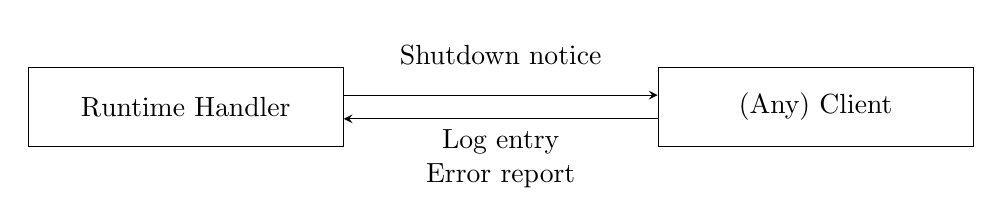
\begin{tikzpicture}[->, >=stealth, rectangle, every node/.style={minimum height=1cm, minimum width=4cm}, node distance=8cm, auto]
			
				\node [draw] (H) {Runtime Handler};
				\node [draw] (C) [right of = H] {(Any) Client};

				\draw [transform canvas={yshift=0.15cm}] (H) edge node[above, align=center]
				{Shutdown notice} (C);
				
				\draw [transform canvas={yshift=-0.15cm}] (C) edge node[below, align=center]
				{Log entry\\Error report} (H);
				
			\end{tikzpicture}
			\caption*{\emph{Possible simple messages between handler and bot- or engine client}}
		\end{figure}
		
		\begin{figure}[H]
			\centering
			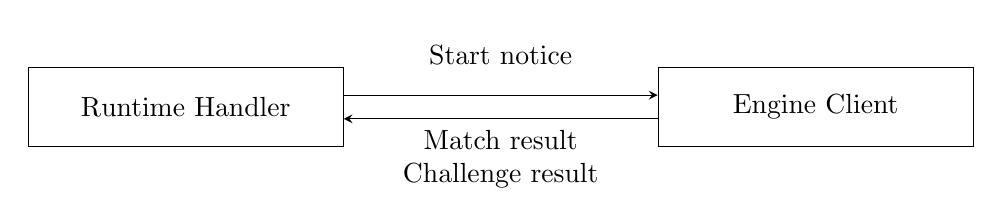
\begin{tikzpicture}[->, >=stealth, rectangle, every node/.style={minimum height=1cm, minimum width=4cm}, node distance=8cm, auto]
			
				\node [draw] (H) {Runtime Handler};
				\node [draw] (EC) [right of = H] {Engine Client};

				\draw [transform canvas={yshift=0.15cm}] (H) edge node[above, align=center]
				{Start notice} (EC);
				
				\draw [transform canvas={yshift=-0.15cm}] (EC) edge node[below, align=center]
				{Match result\\Challenge result} (H);
				
			\end{tikzpicture}
			\caption*{\emph{Possible simple messages between handler and engine client}}
		\end{figure}
		
			\paragraph{Start notice}
			
			This message is only sent once per game to the engine client, as a signal that all actor clients have received all the data (api and actor binaries) that they needed to start working, and a game may be started. Following its reception, the engine client starts the game by invoking the engine object's \code{playGame} method.
		
			\paragraph{Shutdown notice}
			
			This message can be sent at any time during the game, and signals its end --- either due to some error happening or normal game completion --- to the clients, who after receiving it should finish all running tasks, and stop themselves.
		
			\paragraph{Log entry}
			
			Log messages are the only non-control messages, due to them not affecting the flow of the game in any way. They carry their target (the actor or actors whose log will contain the message) and their message itself as their payload. They are sent at any time by one of the actor clients, and are processed independently of the control messages by the runtime handler.
			
			\paragraph{Error report}
			
			Much like log entries, error reports can be sent at any time; however, instead of being actor initiated, they are generated by the client runtime if any irregularity has happened. They can be caused by execptions thrown in the actors' code, unexpected runtime behavior, or attempted access to guarded resources by the actor. As they signal unrecoverable errors, the runtime handler will interrupt the game after receiving them, and choose a result fitting the context the report was created in and the information it carries.
			Based on these pieces of information, the handler will generally mark the game as ended with:
			
			\begin{itemize}
				\item An error caused defeat of the bot of the report's sender (e.g. in case of attempted permission violation or general exception in the bot's code).
				
				\item An error (no winner or loser) if the error occurred not in the actor's, but in the runtime's code
				
				\item Game error if the report was sent from the engine's client due to the former's failure. 
			\end{itemize}
			
			\paragraph{Match result, Challenge result}
			
			Signals from the engine client that imply the engine object's \code{playGame} method successfully finished. They carry the data containing the game's result in accordance with the game model's description. If no error has happened, they act as the signal for the end of the game, and as such may be viewed to form a non-simple message pair with start notice.
			
		\subsection*{Actor binary transfer}
		
		Actor binary messages serve as both parts of a request--response pair. When making a request, a client asks the handler for a type of binary resource required to do its job --- the game's api, engine, or the managed bot. The handler in return sends back the requested binary, while also keeping track of all such requests. If all needed binaries have been sent to all clients, the handler will initialize the start of the game using a start notice message. 
		
		\begin{figure}[H]
			\centering
			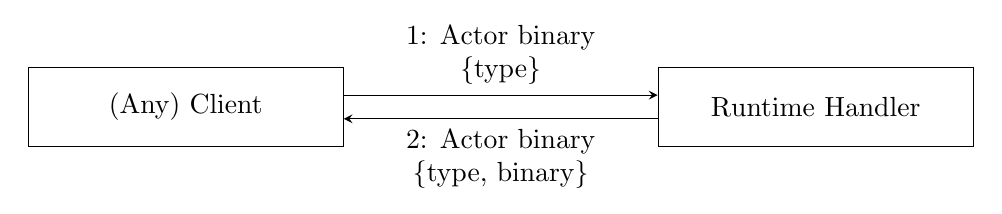
\begin{tikzpicture}[->, >=stealth, rectangle, every node/.style={minimum height=1cm, minimum width=4cm}, node distance=8cm, auto]
			
				\node [draw] (C) {(Any) Client};
				\node [draw] (H) [right of = C] {Runtime Handler};

				\draw [transform canvas={yshift=0.15cm}] (C) edge node[above, align=center]
				{1: Actor binary\\\{type\}} (H);
				
				\draw [transform canvas={yshift=-0.15cm}] (H) edge node[below, align=center]
				{2: Actor binary\\ \{type, binary\} } (C);
				
			\end{tikzpicture}
			\caption*{\emph{Actor binary request--response}}
		\end{figure}
		
		\subsection*{Remote invocation}

		Remote invocation is the most complex communication operation as it involves routing by the handler, and multiple possible valid return types.
		
		As the engine runtime's proxy captures a method call attempt by the engine object, the client sends a proxy call message containing the target bot, requested method identifier, and optional method parameters. This message is forwarded by the handler to the target client, who executes its bot's appropriate method. If this method produces a valid result under the configurable time limit, that value is returned wrapped into a call result message, all the way to the engine. If some error happens during the evaluation, (as usual) an error report is returned to the handler.
		
		However, a special case is also possible, if the bot's method does not finish in time. If this happens, instead of an error report, a bot timeout message is sent back to the engine. This bot timeout acts as a 'recoverable error' --- an event when the engine can choose to ignore the bot's shortcoming. If the engine was created without support for these occurrences, the default error processing takes place.
		
		\begin{adjustwidth}{-0.8cm}{}
		\begin{minipage}[t]{.45\textwidth}
			\begin{figure}[H]
				\centering
				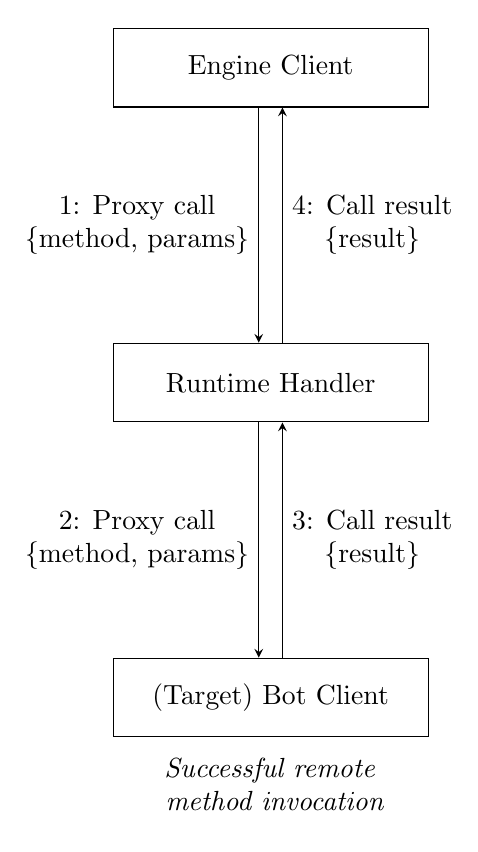
\begin{tikzpicture}[->, >=stealth, rectangle, every node/.style={minimum height=1cm, minimum width=4cm}, node distance=8cm, auto]
			
					\node [draw] (E) {Engine Client};
					\node [draw] (H) [below of = E, node distance=4cm] {Runtime Handler};
					\node [draw] (B) [below of = H, node distance=4cm] {(Target) Bot Client};

					\draw [transform canvas={xshift=-0.15cm}] (E) edge
					node[left, align=center, minimum width=0cm]
					{1: Proxy call \\ \{method, params\}} (H);
				
					\draw [transform canvas={xshift=0.15cm}] (H) edge
					node[right, align=center, minimum width=0cm]
					{4: Call result \\ \{result\}} (E);
				
					\draw [transform canvas={xshift=-0.15cm}] (H) edge
					node[left, align=center, minimum width=0cm]
					{2: Proxy call \\ \{method, params\}} (B);
				
					\draw [transform canvas={xshift=0.15cm}] (B) edge
					node[right, align=center, minimum width=0cm]
					{3: Call result \\ \{result\}} (H);
				
					\node [node distance=1.1cm, align=center] () [below of = B]
					{\emph{Successful remote} \\ \emph{ method invocation}};
				
				\end{tikzpicture}
			\end{figure}
		\end{minipage}\hfill
		\begin{minipage}[t]{.45\textwidth}
			\begin{figure}[H]
				\centering
				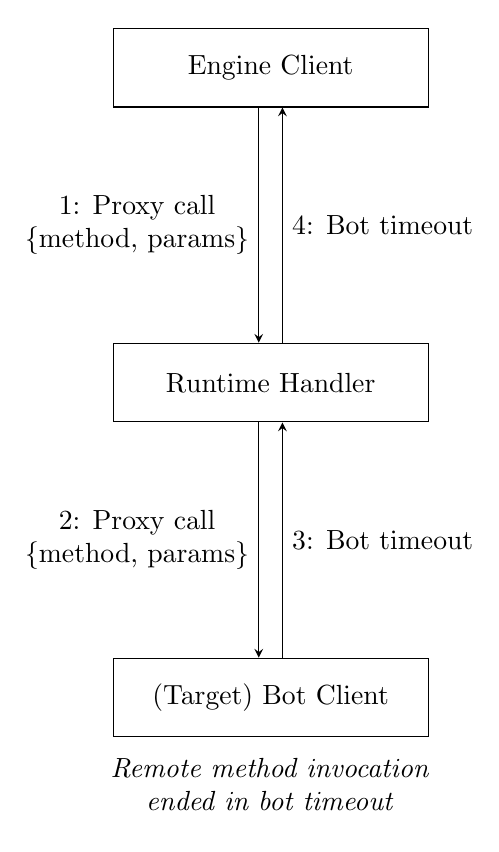
\begin{tikzpicture}[->, >=stealth, rectangle, every node/.style={minimum height=1cm, minimum width=4cm}, node distance=8cm, auto]
			
					\node [draw] (E) {Engine Client};
					\node [draw] (H) [below of = E, node distance=4cm] {Runtime Handler};
					\node [draw] (B) [below of = H, node distance=4cm] {(Target) Bot Client};

					\draw [transform canvas={xshift=-0.15cm}] (E) edge
					node[left, align=center, minimum width=0cm]
					{1: Proxy call \\ \{method, params\}} (H);
			
					\draw [transform canvas={xshift=0.15cm}] (H) edge
					node[right, align=center, minimum width=0cm]
					{4: Bot timeout} (E);
			
					\draw [transform canvas={xshift=-0.15cm}] (H) edge
					node[left, align=center, minimum width=0cm]
					{2: Proxy call \\ \{method, params\}} (B);
			
					\draw [transform canvas={xshift=0.15cm}] (B) edge
					node[right, align=center, minimum width=0cm]
					{3: Bot timeout} (H);
				
					\node [node distance=1.1cm, align=center] () [below of = B]
					{\emph{Remote method invocation} \\ \emph{ended in bot timeout}};
				
			\end{tikzpicture}
			\end{figure}
		\end{minipage}
		\end{adjustwidth}

%\end{document}








%----------------------------------------------------------------------------
\chapter*{Köszönetnyilvánítás}\addcontentsline{toc}{chapter}{Köszönetnyilvánítás}
%----------------------------------------------------------------------------

Ez nem kötelezõ, akár törölhetõ is. Ha a szerzõ szükségét érzi, itt lehet köszönetet nyilvánítani azoknak, akik hozzájárultak munkájukkal ahhoz, hogy a hallgató a szakdolgozatban vagy diplomamunkában leírt feladatokat sikeresen elvégezze. A konzulensnek való köszönetnyilvánítás sem kötelezõ, a konzulensnek hivatalosan is dolga, hogy a hallgatót konzultálja.

%\listoffigures\addcontentsline{toc}{chapter}{Ábrák jegyzéke}
%\listoftables\addcontentsline{toc}{chapter}{Táblázatok jegyzéke}

\bibliography{mybib}
\addcontentsline{toc}{chapter}{Irodalomjegyzék}
\bibliographystyle{plain}

%----------------------------------------------------------------------------
\appendix
%----------------------------------------------------------------------------
\chapter*{Függelék}\addcontentsline{toc}{chapter}{Függelék}
\setcounter{chapter}{6}  % a fofejezet-szamlalo az angol ABC 6. betuje (F) lesz
\setcounter{equation}{0} % a fofejezet-szamlalo az angol ABC 6. betuje (F) lesz
\numberwithin{equation}{section}
\numberwithin{figure}{section}
\numberwithin{lstlisting}{section}
%\numberwithin{tabular}{section}

%----------------------------------------------------------------------------
\section{A TeXnicCenter felülete}
%----------------------------------------------------------------------------
\begin{figure}[!ht]
\centering
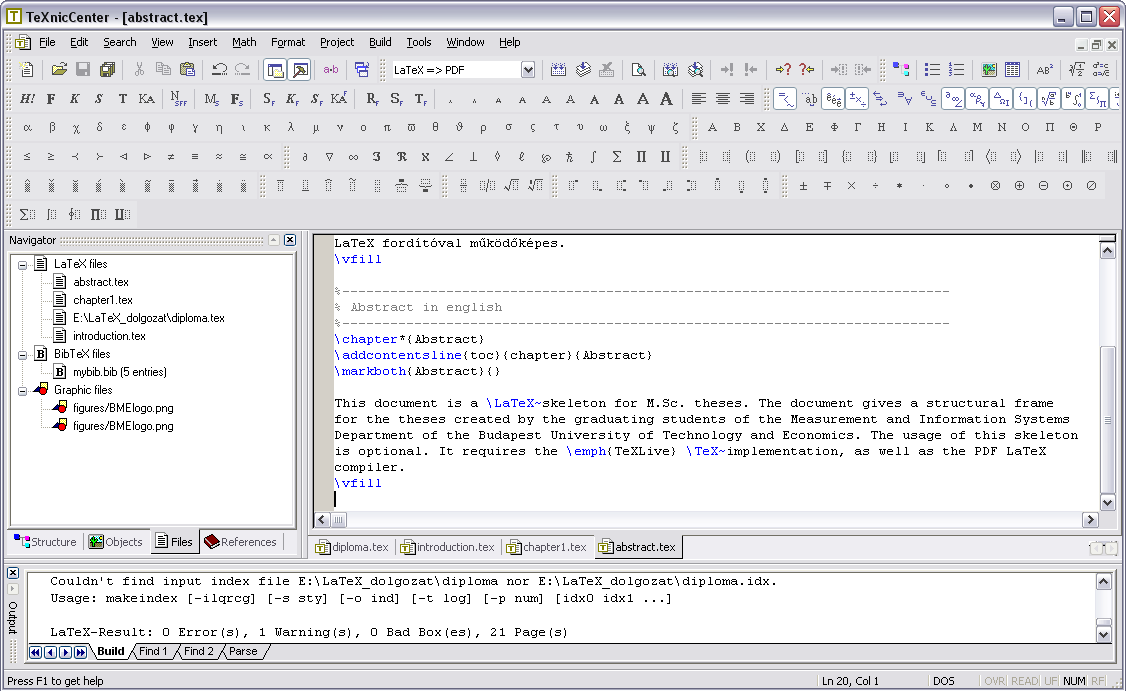
\includegraphics[width=150mm, keepaspectratio]{figures/TeXnicCenter.png}
\caption{A TeXnicCenter Windows alapú \LaTeX-szerkesztõ.} 
\end{figure}

%----------------------------------------------------------------------------
\clearpage\section{Válasz az ,,Élet, a világmindenség, meg minden'' kérdésére}
%----------------------------------------------------------------------------
A Pitagorasz-tételbõl levezetve
\begin{align}
c^2=a^2+b^2=42.
\end{align}
A Faraday-indukciós törvénybõl levezetve
\begin{align}
\rot E=-\frac{dB}{dt}\hspace{1cm}\longrightarrow \hspace{1cm}
U_i=\oint\limits_\mathbf{L}{\mathbf{E}\mathbf{dl}}=-\frac{d}{dt}\int\limits_A{\mathbf{B}\mathbf{da}}=42.
\end{align}







\label{page:last}
\end{document}
